\documentclass[border=4pt]{standalone}
% Preámbulo común de las figuras. Cada figura es un documento standalone
% que se compila a SVG con scripts/build_figures.sh
\usepackage[utf8]{inputenc}
\usepackage{amsmath}
\usepackage{tikz}
\usepackage[american, siunitx]{circuitikz}
\usetikzlibrary{arrows.meta,calc,decorations.pathmorphing,patterns}
\tikzset{
  >={Stealth[length=2.2mm]},
  eje/.style={->, thin},
  hilo/.style={thick},
}
% Paleta común: tonos medios legibles sobre fondo claro
\definecolor{azul}{RGB}{31,94,168}
\definecolor{rojo}{RGB}{192,57,43}
\definecolor{verde}{RGB}{39,128,73}
\definecolor{naranja}{RGB}{211,120,30}
\definecolor{morado}{RGB}{125,60,152}

\begin{document}
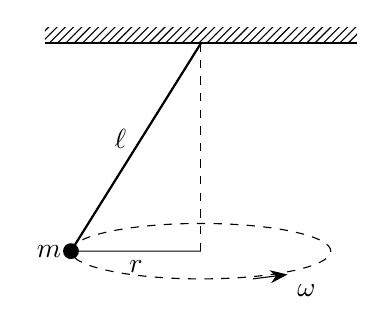
\begin{tikzpicture}[scale=1.1]
  \fill[pattern=north east lines] (-1.8,0) rectangle (1.8,0.18);
  \draw[thick] (-1.8,0) -- (1.8,0);
  \coordinate (O) at (0,0);
  \coordinate (C) at (0,-2.4);
  \draw[dashed] (C) ellipse (1.5 and 0.32);
  \draw[dashed] (O) -- (C);
  \draw[hilo] (O) -- (-1.5,-2.4);
  \draw[thin] (C) -- node[below]{$r$} (-1.5,-2.4);
  \fill (-1.5,-2.4) circle (2.6pt) node[left]{$m$};
  \draw[->] (0.6,-2.72) -- (1.0,-2.67) node[below right]{$\omega$};
  \node[left] at (-0.75,-1.1) {$\ell$};
\end{tikzpicture}
\end{document}
